\documentclass[11pt]{article}
\usepackage[french]{babel}
\usepackage[T1]{fontenc}
\usepackage{fontspec}
\usepackage[utf8]{inputenc}
\usepackage{url}
\usepackage{eurosym}
\usepackage{pdfpages}
\usepackage{ulem} % to use a strikeout/strikethrough font
\usepackage{color}
\newcommand{\fs}[1]{\textcolor{red}{\sout{#1}}}
\newcommand{\f}[1]{\textcolor{blue}{#1}}
\usepackage{graphicx} % Inclure des images
\usepackage{multicol} % Multi-colonnes


\usepackage[autolanguage, np]{numprint} % écriture des virgules
\usepackage[top=3cm,right=2cm,bottom=2cm,left=2cm]{geometry}

\title{HAUM}
\author{Assemblées Générales Ordinaire \& Extraordinaire}
\date{6 Février 2018}

\begin{document}
\maketitle


\section*{Convocation}

Madame, Monsieur,

L'association HAUM vous convoque à ses Assemblées Générales Ordinaire \& Extraordinaire qui se tiendront le :

\begin{center}
{\Large 6 Février 2018 à 19h00}\\
à la Ruche Numérique,\\19 Bd M\&A Oyon au 1\textsuperscript{er} étage,\\72 100 Le Mans
\end{center}

En cas d'impossibilité, veillez vous faire excuser et vous faire représenter si vous le souhaitez (2 procurations maximum par personne présente, Statuts, art. 6).

\vspace{1.5cm}

\hrule
\vspace{.3cm}
\begin{center}
\Large\bfseries Assemblée Générale Extraordinaire
\end{center}
\vspace{.3cm}
\hrule

\vspace{1.5cm}

\section*{Déroulement}

\begin{enumerate}
    \item Appel et annonce des procurations
\end{enumerate}

\section*{Clotûre}

\vspace{1.5cm}

\hrule
\vspace{.6cm}
\begin{center}
\Large\bfseries Assemblée Générale Ordinaire
\end{center}
\vspace{.3cm}
\hrule

\vspace{1.5cm}

\section*{Déroulement}

\begin{enumerate}
    \item Présentation de l'association
    \item Rapport moral
        \begin{enumerate}
            \item Bilan
            \item Objectifs
            \item Questions
        \end{enumerate}
    \item Rapport financier
        \begin{enumerate}
            \item Bilan \& Objectifs
            \item Previsionnel 2018
            \item Questions
        \end{enumerate}
    \item Motions et vote
    \item Election du nouveau bureau
    \item Questions diverses
\end{enumerate}

\section{Présentation de l'association}

\section{Rapport Moral}

\subsection{Bilan}

\subsection{Le Mans Innovation \& déménagement}
Une fois de plus, l'année passée a été riche en changements, projets et évènements. Au
premier plan, il faudra retenir de 2017 qu'elle fut une année de déménagement. Le HAUM
quitte ainsi le 19 Boulevard Oyon pour prendre ses quartiers au 57 Boulevard Demorieux, au
sein de Le Mans Innovation (LMI).
Le nouveau local comprend deux salles pour un total d'environ 120m\textsuperscript{2}. La
plus grande des deux accueil un espace "propre" comprenant entre autres la paillasse
électrique, le Free to Hack et une vitrine permettant de présenter les activités. Le
second (atelier "sale") accueille le stock de matières premières, la fraiseuse, les scies & perceuses.

Dans le cadre de LMI, l'espace fablab (occupé par le HAUM) a été équipé
d'une découpeuse LASER (Robotseed, 600\times400mm de surface utile) et d'une imprimante 3D
(Ultimaker 2+ Extended). Ces équipements sont à disposition du HAUM et leur maintenance
sous sa responsabilité.

Des partenariats avec des résidents de LMI ont vu le jour, le local est ainsi utilisé en
journée par Bertrand (Chaines de Pluie, atelier propre) et Marc (Furion Motorcycles,
atelier salle). Divers ajustements quant au partage des tâches sont à prévoir dans
l'avenir pour que le local reste propre et soit utilisé au mieux, toutefois, ces
rapprochements sont prometteurs.

Reste à définir également les modalités de contrôle de l'accès au local. La présence de
matériel dangereux pose la question de comment limiter le risque de blessures et préserver
les machines. Lors de plusieurs discussions en séance, il a été convenu de mettre en place
un contrôle d'accès au local par badge. Il s'agit d'un projet en cours de réalisation
prévu pour une installation au plus tôt. Dans le cadre de la protection du matériel il a
également été évoqué de changer les canons : des doutes planent sur d'éventuels doubles
des clés ayant pu être réalisés sans le consentement du HAUM ou de LMI.

Dans cette fin d'exercice, le bureau du HAUM s'est attaché à réguler l'accès de personnes
non membres aux machines et au lieu suite à de sérieux doutes sur les activités de
certains (d'un point de vue légal entre autres).

\subsection{Evènements}

Le HAUM a cette année encore participé à de nombreux évènements et proposé autant de
projets innovants. Voici les plus marquants.

\paragraph{HAMExpo} Sur une invitation de l'Électrolab (Nanterre), le HAUM a participé à
HAMExpo, salon de radioamateurs organisé au Mans en 2018. Les membres présents ont pu
échanger avec la communauté des RA et avec quelques membres de l'Électrolab.

\paragraph{Festival D} L'édition 2017 du festival était organisé par Ping et l'ESBA-TALM
au Quai d'Angers. Elle a rassemblé de nombreuses structures présentant des projets
innovants allant de la tricoteuse numérique à l'opendata musicale en passant par divers
robots et machines. Le HAUM présentait alors un remix du dHAUM/dHAUMidi ... appelé
dHAUMadi (désolé). Le projet avait été prévu pour n'être pas d'un niveau technique trop
élevé afin de permettre à de nouveaux membres de s'impliquer dans la vie de l'association.
Malgré ce point, le projet n'avançant pas, les mêmes membres que d'habitude se sont
attelés à la tâche et ont réussi à produire un jeu à taille humaine très apprécié du
public. Merci à eux !

\paragraph{Teriaki} Le festival Teriaki s'est, comme à l'accoutumée, déroulé à la fin
août.

\paragraph{24h du code}

TODO

\subsection{Projets et axes}

\subsection{Objectifs}

L'année 2016 a vu naître et progresser bon nombre de partenariats et de discussion. Il est donc raisonnable d'espérer que 2017 apportera son lot de nouveau matériel et de nouvelles relations.

Il est temps également de travailler sur l'axe de mutualisation des moyens pour que chacun des membres puisse réaliser ses envies et qu'un minimum d'argent soit perdu en doublons.

Le déménagement a entrainé la perte de l'accès à Internet et il est également nécessaire de remédier à cela dans les mois à venir pour garantir à tous un accès convenable aux ressources.

Les prestations et actions extérieures sont bien sûr à poursuivre et à encourager. Il faudra par ailleurs simplifier les relations avec les partenaires afin d'éviter les malentendus encore trop courants. La réalisation de prestations contribue au financement de l'association et il est souhaitable qu'un maximum de membres y participent.

Enfin, parce que l'association compte toujours plus de membres, il faudra travailler à l'amélioration des locaux pour permettre de l'utiliser comme lieu de travail bien sûr mais également comme lieu de vie et d'échange. Le HAUM vise à proposer une vision alternative du rapport à la technologie et si cela passe bien sûr par les aspects techniques, cela peut également être renforcé par des temps d'échanges informels (Jeudi du Libre) ou non (HAUMTalks).

\section{Rapport financier}

\subsection{En images}
Nous présentons ici un focus des comptes à la date d'aujourd'hui. Le bilan financier
sera présenté au début de l'année 2017 par mail. Cela permettra d'établir les comptes
au 31 décembre.
\begin{center}
\begin{multicols}{2}
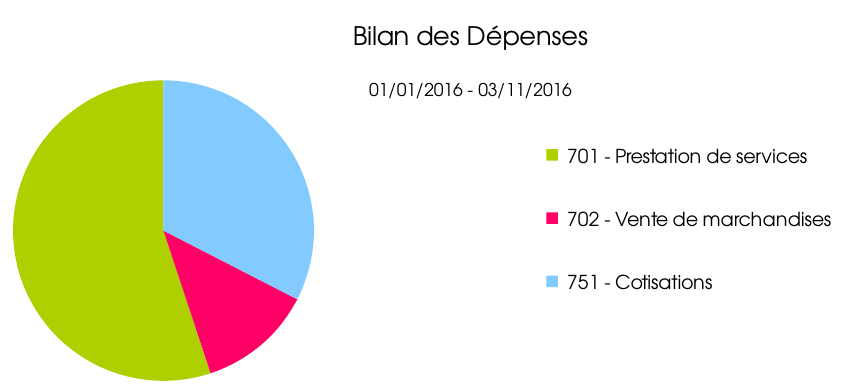
\includegraphics[width=8cm]{1DossierAGRecettes.png}

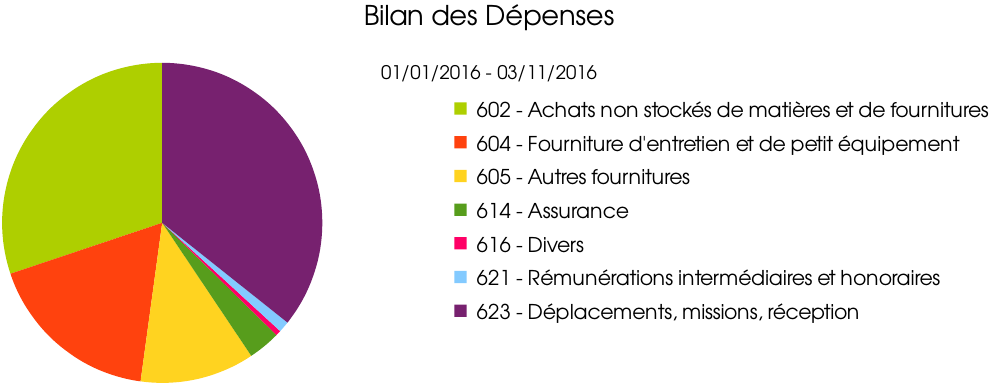
\includegraphics[width=8cm]{2DossierAGDepenses.png}
\end{multicols}

\begin{multicols}{2}
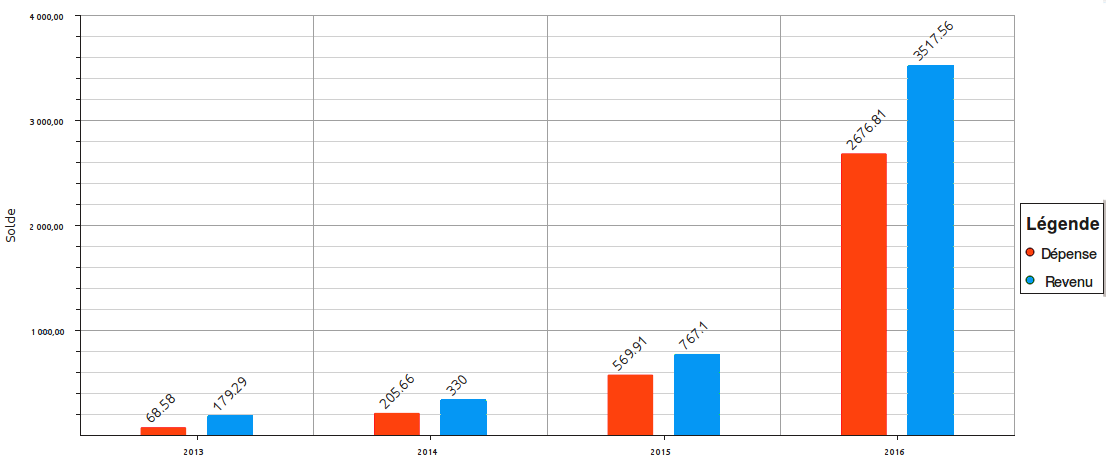
\includegraphics[width=8cm]{3DossierAGGeneral.png}

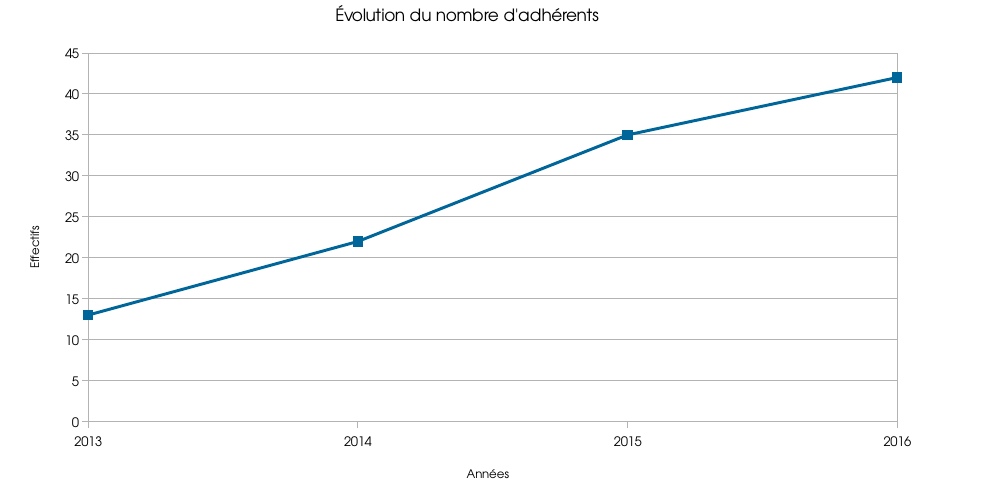
\includegraphics[width=8cm]{4DossierAGAdherents.png}
\end{multicols}
\end{center}
\subsection{Bilan et objectifs}
L'ensemble des comptes de l'association depuis sa création a été repris de manière
à obtenir une tenue de comptes exacte et conforme au Plan Comptable Général français.

Nous pouvons alors remarqué que les volumes financiers sont en forte croissance
cette année.

L'année dernière nous avions pour objectif la mutualisation des moyens matériel.
On progresse bien dans cette voie : il nous a été possible d'acheter une perceuse à
colonne, un \textit{plotter} de découpe et un jeu de tournevis.
Il est maintenant possible de gérer le consommable sans difficulté et d'assumer dans
une moindre mesure le besoin en trésorerie pour la réalisation des projets pour lesquels
une rétribution nous est donnée.

Si on souhaite être en capacité de financer des machines ou de l'outillage plus onéreux
ou en plus grand nombre, l'augmentation des cotisations, des mécénats et/ou des
actions qui seraient capables de nous rapporter de l'argent serait la bienvenue.

\bigskip

Cette année encore des difficultés de gestion de trésorerie ont été rencontrées. Ce qui
nous amène à réaffirmer les règles instaurées l'an passé :
\begin{itemize}
 \item Toutes les factures doivent être établies \textbf{au nom du HAUM} et ne
 contenir que des éléments \textbf{achetés pour le HAUM}.
 \item Les dépenses de l'argent du hackerspace ne doivent être faites qu'après
 \textbf{consultation des autres membres} et, surtout, \textbf{vérification de la
 trésorerie}.
\end{itemize}
De plus, les dépenses augmentant significativement, avant toute dépense d'argent, une
demande de validation \textbf{par mail} devra désormais être effectuée.

Le focus financier contient, à ce jour, un impayé de 250\euro concernant un chèque refusé
à trois reprises. Des démarches sont actuellement en cours pour y remédier.

\subsection{Prévisions 2017}

Pour l'année à venir, le budget prévisionnel a été construit sur la base des charges
et des recettes de l'année 2016.

\subparagraph{Recettes}
Il est estimé pour les recettes :
\begin{itemize}
 \item 437,31~\officialeuro{} de prestations ;
 \item 170~\officialeuro{} de vente de marchandises ;
 \item \np{1377,60}~\officialeuro{} de cotisations ;
 \item \np{8966}~\officialeuro{} de subvention exceptionnelle pour l'achat d'une découpeuse laser.
\end{itemize}

\subparagraph{Charges}
Pour les charges, il est prévu :
\begin{itemize}
 \item 260~\officialeuro{} pour l'achat de fournitures ;
 \item 508,03~\officialeuro{} pour les petits équipements ;
 \item 246~\officialeuro{} pour les autres fournitures (par exemple, en 2016, les tee-shirts) ;
 \item 150~\officialeuro{} pour la communication (cartes de visites, ...) ;
 \item 450~\officialeuro{} pour les frais de déplacement, de réception, ... ;
 \item 239,88~\officialeuro{} pour une connection internet indépendante ;
 \item \np{8966}~\officialeuro{} achat de la découpeuse laser.
\end{itemize}

\subparagraph{Bénévolat}La valorisation du bénévolat sera établie régulièrement lors des réunions mensuelles.
Elle a été estimée à \np{8142}~\officialeuro{} pour l'année prochaine.

\subparagraph{}Le budget prévisionnel est alors de \np{28392,91}~\officialeuro{}.

\section{Motions}
Aucun amendement au Règlement Intérieur n'a été proposé.

\section{Questions Diverses}

\newpage

\clearpage
\thispagestyle{empty}
\topskip0pt
\vspace*{\fill}
\begin{center}
\hrule
\vspace{.3cm}
\Huge\bfseries Annexes
\vspace{.3cm}
\hrule
\vspace{2cm}
\Large
\noindent Bilan Financier 2016\\
Bilan Général 2013-2016\\
Budget Prévisionnel 2017
\end{center}
\vspace*{\fill}

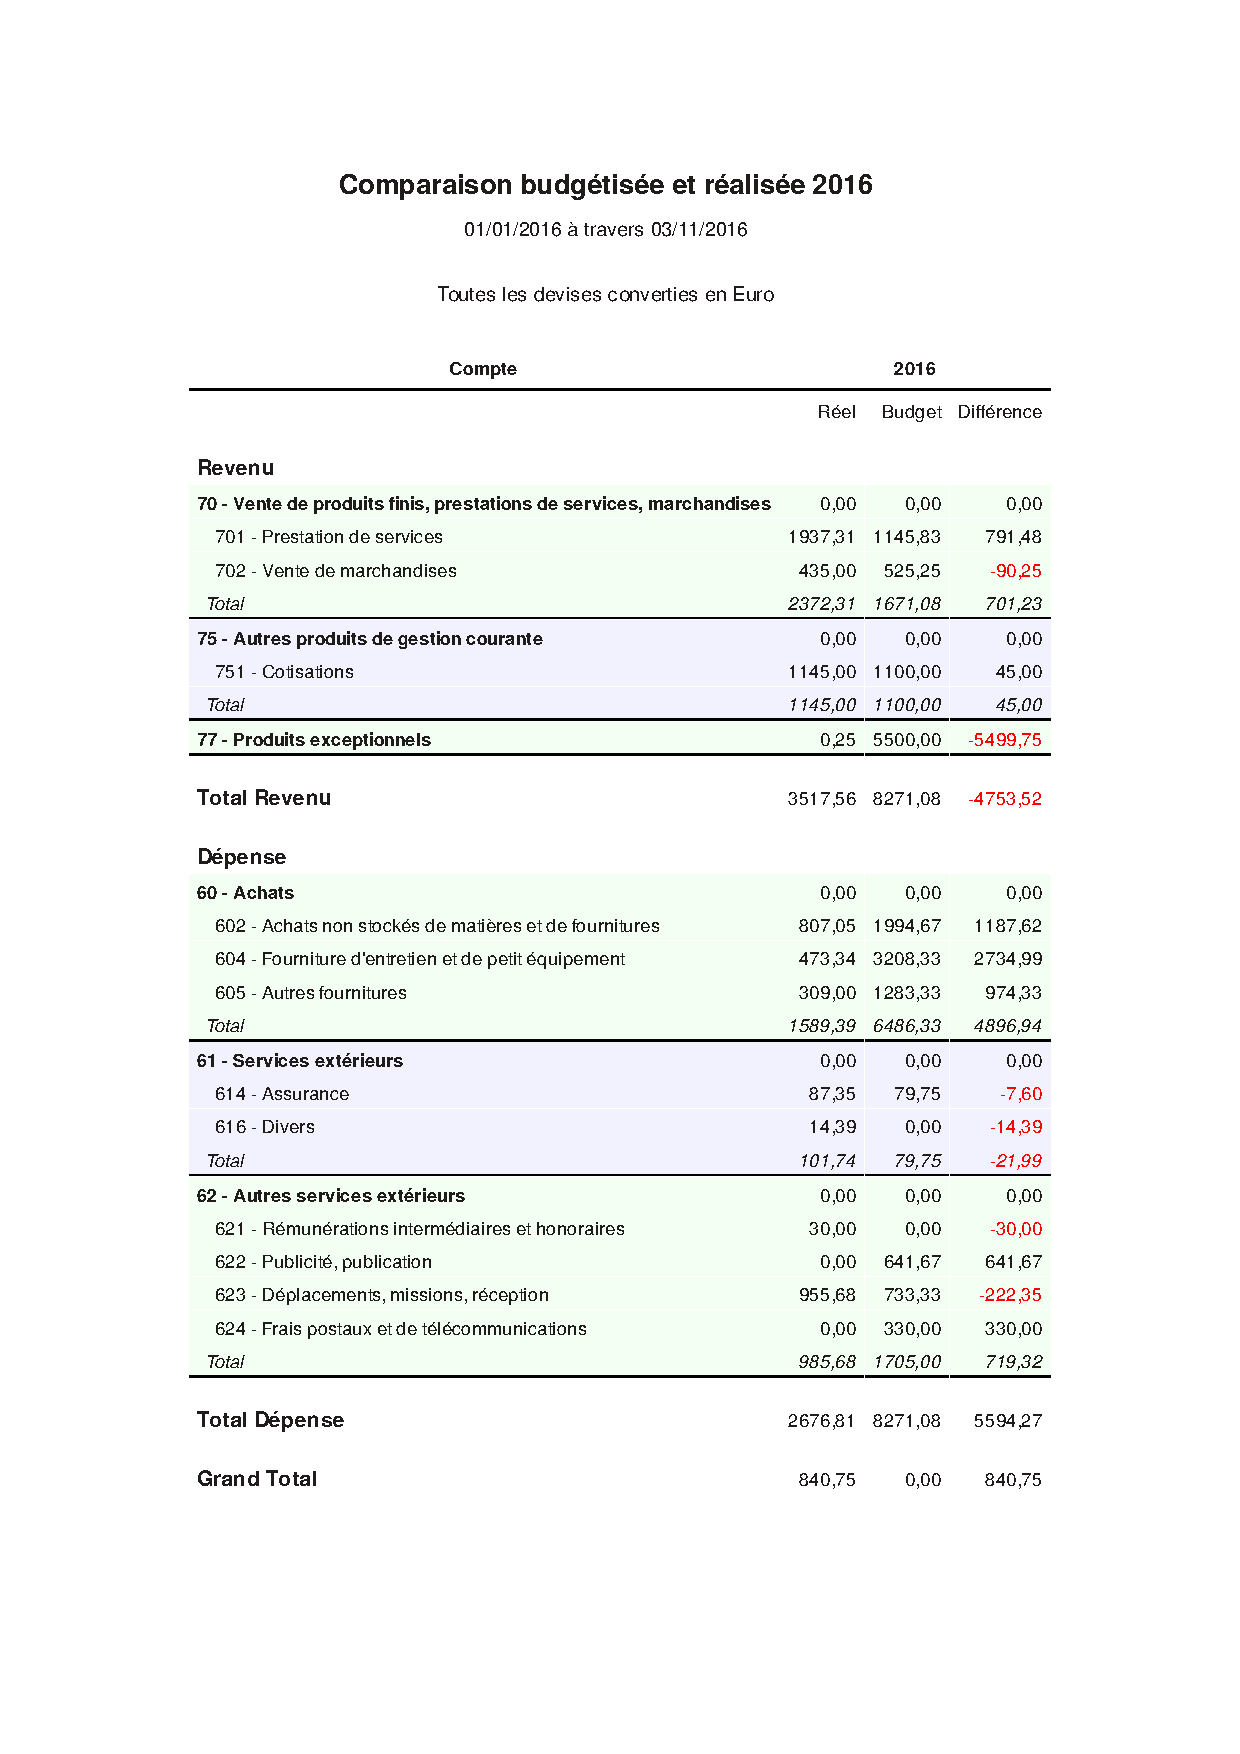
\includepdf[pages=-]{BilanFinancier2016.pdf}
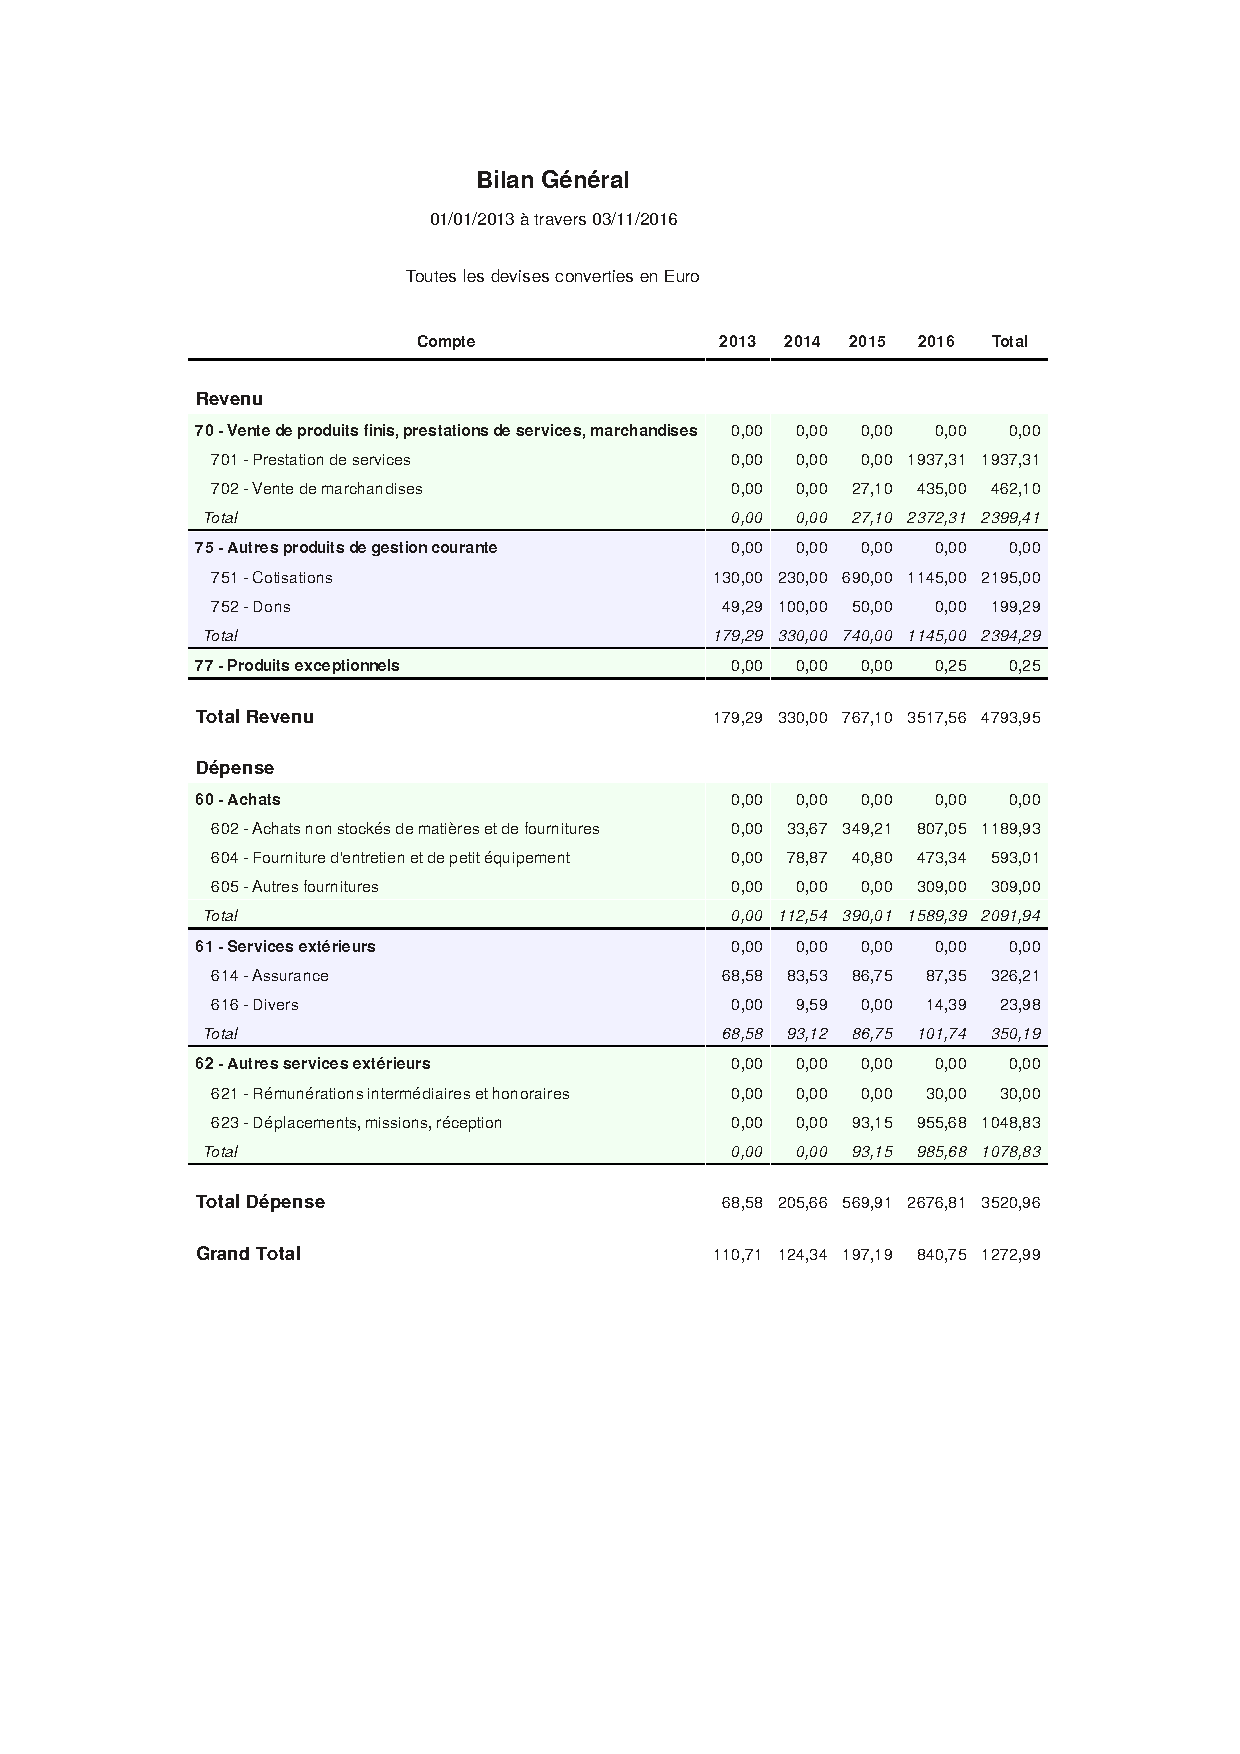
\includepdf[pages=-]{BilanGeneral2016.pdf}
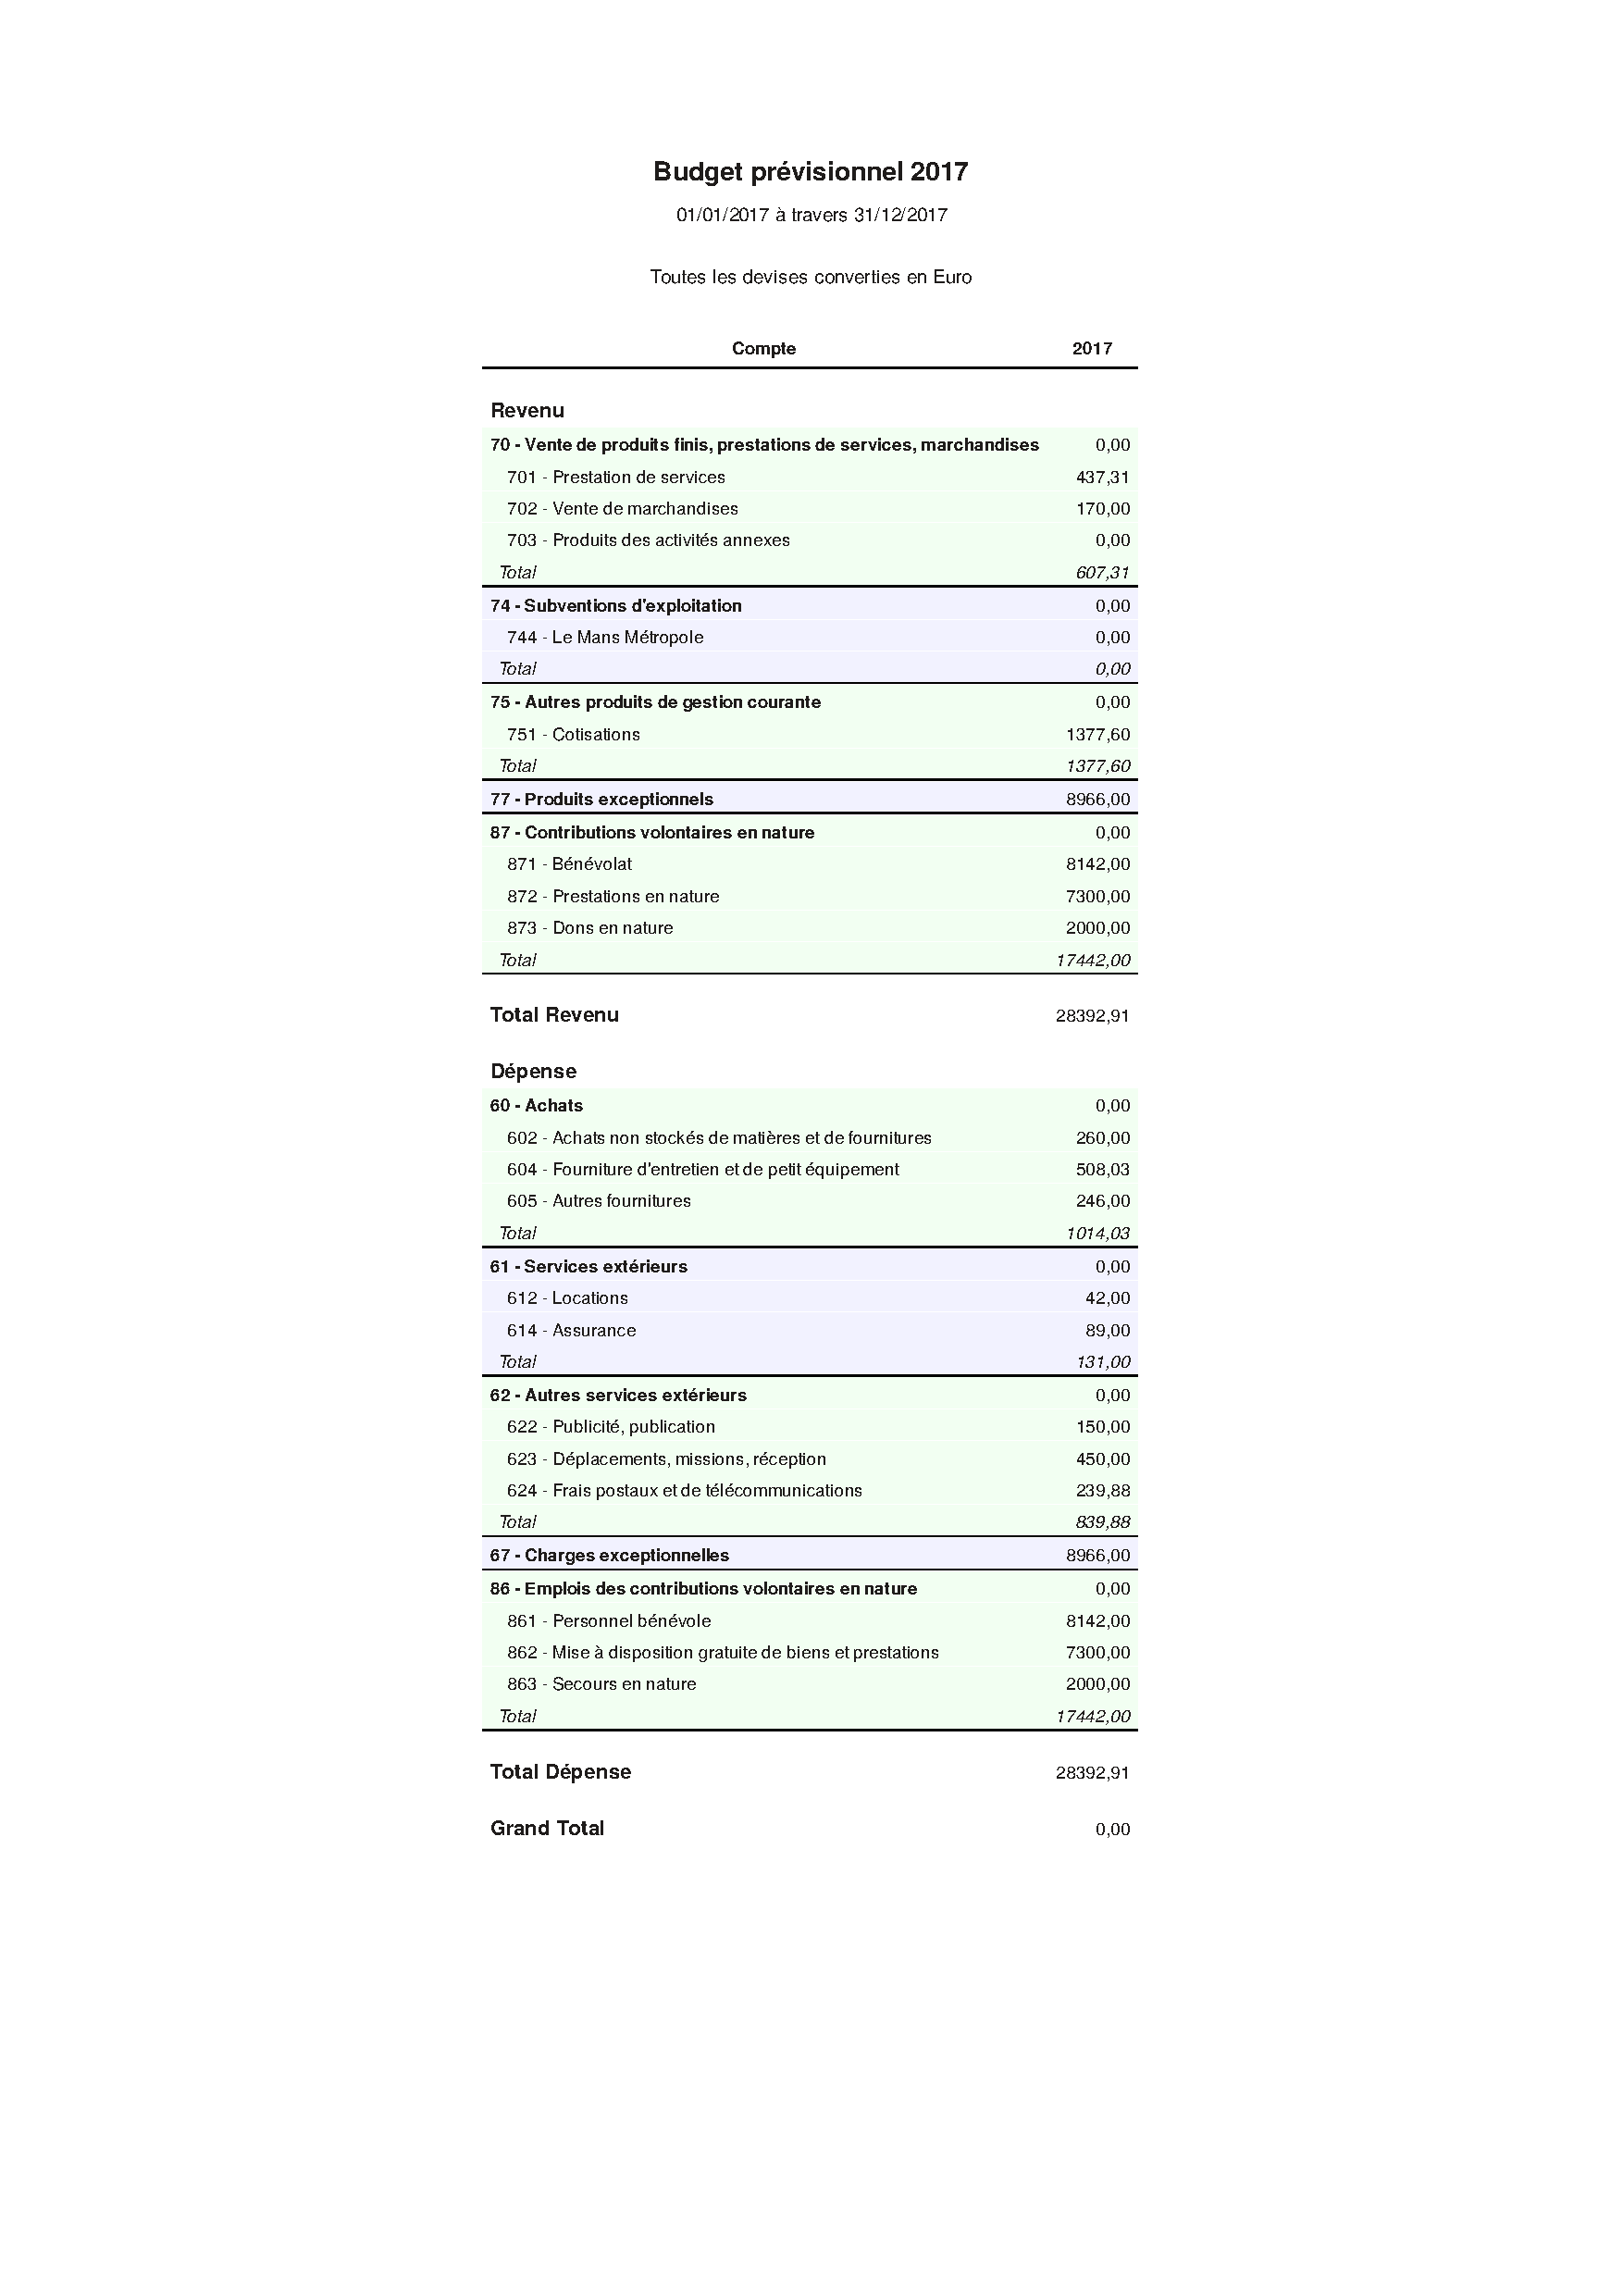
\includepdf[pages=-]{BudgetPrevisionnel2017.pdf}

\end{document}
